% Copyright 2026 Sreeram Anil
% SPDX-License-Identifier: CC-BY-4.0
% =============================================================================
%  Luenberger observer (deterministic-observer family)
% =============================================================================
\chapter{Luenberger Observer with Gain Scheduling (Luenberger)}
\label{ch:luenberger}

\section*{At a glance}
\begin{tabular}{@{}l>{\raggedright\arraybackslash}p{0.76\textwidth}@{}}
Family & Deterministic observers \\
Header & \texttt{include/estkit/observers/luenberger.hpp} \\
Registered name & \texttt{Luenberger} \\
State dimension & $n_x = 4$ (cell model) --- generic in $n_x, n_u, n_y$ \\
Cost per step & $\mathcal{O}(n_x^3)$ only when the gain is re-designed; $\approx 0.5\,\mu$s/step measured, no heap \\
Primary references & \cite{luenberger1964,luenberger1971,ackermann1972,ogata2010,franklin1998digital} \\
\end{tabular}

\section{Motivation and aerospace/BMS relevance}
The Kalman filter answers the state-estimation problem in a stochastic setting: it needs
$\mQ$ and $\mR$, it propagates a covariance, and its optimality claim is only as good as those
two matrices.  A battery-management unit in an eVTOL aircraft rarely knows them.  The current
sensor has a specification, not a covariance; the hysteresis model error is a bounded modelling
artefact, not white noise; and the certification argument that matters for
DO-311A-class equipment \cite{rtca2017do311a} is \emph{``the estimate converges and stays
bounded''}, not ``the estimate is minimum-variance''.

The Luenberger observer \cite{luenberger1964,luenberger1971} answers exactly that question.  It
replaces the Riccati equation by a single design decision --- where to put the error-dynamics
poles --- and then runs a fixed, pre-computed gain.  There is no covariance to propagate, no
matrix to keep positive definite, and no possibility of covariance collapse.  For a flight
computer this is attractive for three reasons: the run-time code is a matrix--vector product;
the worst-case execution time is trivially bounded; and the design itself is auditable, because
``the SOC error decays with a 60\,s time constant'' is a statement a systems engineer can check
against the mission profile.

The observer is also the structural parent of the rest of this family.  The
proportional-integral observer (\Cref{ch:piobserver}), the sliding-mode observers
(\Cref{ch:smo,ch:supertwistingsmo}), the high-gain observer (\Cref{ch:hgo}), the extended-state
observer (\Cref{ch:eso}) and the disturbance observer (\Cref{ch:dob}) all add one term to the
correction (\ref{eq:lue-update}) below; understanding the linear core once is enough to read all
of them.  The same class also provides the \texttt{SSKF} registration (\Cref{ch:sskf}), which
keeps the structure and takes the gain from the algebraic Riccati equation instead.

\section{Problem statement and assumptions}
The plant is the discrete-time nonlinear model of the estimator contract,
\begin{align}
\vx_{k+1} &= f(\vx_k, \vu_k) + \vw_k , \label{eq:lue-plant-f}\\
\vy_k     &= h(\vx_k, \vu_k) + \vv_k , \label{eq:lue-plant-h}
\end{align}
with state $\vx\in\real^{n_x}$, input $\vu\in\real^{n_u}$, measurement $\vy\in\real^{n_y}$, and
$\vw_k$, $\vv_k$ \emph{bounded but otherwise arbitrary} disturbances.  No distributional
assumption is made.  Write
\begin{equation}
\mA_k = \left.\frac{\partial f}{\partial \vx}\right|_{\xhat_k,\vu_k} , \qquad
\mC_k = \left.\frac{\partial h}{\partial \vx}\right|_{\xhat_k,\vu_k} ,
\label{eq:lue-jac}
\end{equation}
the Jacobians evaluated at the current estimate (obtained through \texttt{jac\_F} and
\texttt{jac\_H}, which use the analytic members of the model when they exist and central
differences otherwise).

\begin{assumption}[Detectability]\label{as:lue-detect}
The pair $(\mA_k,\mC_k)$ is detectable at every operating point visited, and observable wherever
pole assignment is used.
\end{assumption}
\begin{assumption}[Slow scheduling]\label{as:lue-slow}
The linearisation \eqref{eq:lue-jac} varies slowly compared with the closed-loop error dynamics,
so that the frozen-time stability analysis is meaningful \cite{shamma1990gain}.
\end{assumption}
\Cref{as:lue-slow} is the one that actually bites on a battery, and \Cref{sec:lue-schedule}
describes what the implementation does when it is violated.

\section{Derivation}

\subsection{Predictor--corrector form and the error dynamics}
The benchmark adapter presents one sample as: a time update with $\vu_{k-1}$, a prior output
prediction, and a measurement update with $(\vy_k,\vu_k)$.  The observer is therefore written in
Franklin's \emph{current-estimator} form \cite[Sec.~8.3]{franklin1998digital}:
\begin{align}
\xminus_k &= f(\xplus_{k-1}, \vu_{k-1}) , \label{eq:lue-predict}\\
\bm{r}_k     &= \vy_k - h(\xminus_k, \vu_k) , \label{eq:lue-resid}\\
\xplus_k  &= \xminus_k + \mL_k \bm{r}_k . \label{eq:lue-update}
\end{align}
Here $\bm{r}_k\in\real^{n_y}$ is the output residual (innovation) and
$\mL_k\in\real^{n_x\times n_y}$ is the observer gain.  Define the estimation error
$\veps_k = \xplus_k - \vx_k$.  Using \eqref{eq:lue-plant-f}--\eqref{eq:lue-plant-h} and the mean
value theorem on $f$ and $h$,
\begin{equation}
\veps_k = (\mI - \mL_k \mC_k)\,\mA_k\, \veps_{k-1}
        + (\mI - \mL_k \mC_k)\,(-\vw_{k-1}) - \mL_k \vv_k
        + \mathcal{O}(\norm{\veps_{k-1}}^2) .
\label{eq:lue-err}
\end{equation}
The observer poles are therefore the eigenvalues of $(\mI - \mL\mC)\mA$, \emph{not} of
$\mA - \mL\mC$.  The two are related: for any square $\bm{M},\bm{N}$, $\operatorname{eig}(\bm{M}\bm{N}) =
\operatorname{eig}(\bm{N}\bm{M})$, hence
\begin{equation}
\operatorname{eig}\big((\mI-\mL\mC)\mA\big) = \operatorname{eig}\big(\mA(\mI-\mL\mC)\big)
= \operatorname{eig}\big(\mA - (\mA\mL)\mC\big) .
\label{eq:lue-currvspred}
\end{equation}
So if $\bar{\mL}$ is the classical \emph{prediction} gain of Luenberger (1971), i.e. the one for
which $\operatorname{eig}(\mA-\bar{\mL}\mC)$ is the desired set, then the current-estimator gain
is
\begin{equation}
\boxed{\ \mL = \mA\inv \bar{\mL} \ }
\label{eq:lue-Lconv}
\end{equation}
This conversion is done once per design and is why the implementation calls
\texttt{solve(A, Lbar)}.

\subsection{Pole assignment by Ackermann's formula}
For $n_y=1$ and $(\mA,\mC)$ observable, Ackermann's formula \cite{ackermann1972},
\cite[Sec.~10-6]{ogata2010} gives the prediction gain in closed form.  With the desired
characteristic polynomial
\begin{equation}
\varphi(z) = \prod_{i=1}^{n_x}(z - p_i) = z^{n_x} + a_{n_x-1}z^{n_x-1} + \dots + a_1 z + a_0 ,
\label{eq:lue-charpoly}
\end{equation}
and the observability matrix $\mathcal{O} = [\mC^\T\ (\mC\mA)^\T\ \cdots\
(\mC\mA^{n_x-1})^\T]^\T$,
\begin{equation}
\bar{\mL} = \varphi(\mA)\,\mathcal{O}\inv \bm{e}_{n_x} ,\qquad
\bm{e}_{n_x} = [0\ \cdots\ 0\ 1]^\T .
\label{eq:lue-ackermann}
\end{equation}
The $z$-plane pole radii are specified directly in \texttt{Options::pole}; a continuous-time
design frequency $\omega_i$ (or time constant $\tau_i = 1/\omega_i$) maps to
\begin{equation}
p_i = e^{-\omega_i \dt} = e^{-\dt/\tau_i} .
\label{eq:lue-polemap}
\end{equation}

\subsection{Why the plain Ackermann formula fails on a finely sampled plant}
\label{sec:lue-cond}
Equation \eqref{eq:lue-ackermann} is exact in real arithmetic and near-useless in floating point
when $\dt$ is small relative to the plant time constants, because the rows of $\mathcal{O}$ are
$\mC, \mC\mA, \mC\mA^2, \ldots$ and $\mA \to \mI$ as $\dt\to 0$: the rows become nearly parallel.
For the 2-RC cell model at $\dt = 0.1$\,s (\Cref{sec:lue-battery}) the measured determinant is
$\det\mathcal{O}\approx 6\times10^{-18}$ with $\norm{\mathcal{O}}_F\approx 2.8$; the
disturbance-augmented versions used in \Cref{ch:eso,ch:dob} reach $\approx 4\times 10^{-30}$.
This is the classical ill-conditioning of single-input pole assignment
\cite{petkov1984poleassignment,kautsky1985robust}.

The implementation removes it exactly.  Since
\begin{equation}
\mA - (\gamma \bar{\mL}')\mC = \gamma\left(\mA' - \bar{\mL}'\mC\right) + \sigma \mI ,
\qquad \mA' \triangleq \frac{\mA - \sigma\mI}{\gamma},
\label{eq:lue-shift}
\end{equation}
assigning the poles $p'_i = (p_i-\sigma)/\gamma$ to the \emph{shifted and scaled} pair
$(\mA',\mC)$ and returning $\bar{\mL} = \gamma\bar{\mL}'$ assigns $p_i$ to the original pair.
Choosing
\begin{equation}
\sigma = \frac{1}{n_x}\sum_i p_i , \qquad
\gamma = \max\Big( |1-\sigma| , \max_i |p_i - \sigma| \Big)
\label{eq:lue-shiftchoice}
\end{equation}
maps the cluster of plant eigenvalues near $1$ onto $\mathcal{O}(1)$-separated values.  Measured
effect on the cell model: the relative error between the achieved and the requested
characteristic polynomial drops from $7\times10^{-9}\ldots5\times10^{-3}$ (plain Ackermann,
worst case at $-10^\circ$C on the augmented pair) to $10^{-16}$ --- machine precision --- at
every operating point tested, and the single-precision build then reproduces the
double-precision benchmark results to three digits.

\subsection{The spread-versus-repeated pole trade-off}
\label{sec:lue-spread}
Pole \emph{assignment} demands that every mode go exactly where it is told.  When two plant
modes are nearly coincident and one of them is weakly observable, separating them costs gain.
For the cell model at $25^\circ$C the open-loop eigenvalues are
$\{1,\,0.9802,\,0.99917,\,0.99847\}$: the slow RC branch and the hysteresis state differ by
$7\times10^{-4}$, and the hysteresis output coefficient is only $M = 5$\,mV.  Requesting the
spread set $\{0.95,0.97,0.99,0.995\}$ is feasible in exact arithmetic but yields
$\norm{\mL}_\infty = 4.2\times 10^{2}$ at $25^\circ$C and $3.5\times 10^{3}$ at $45^\circ$C; the
resulting steady-state SOC standard deviation, computed from the Lyapunov recursion
$\mP = (\mI-\mL\mC)(\mA\mP\mA^\T+\mQ)(\mI-\mL\mC)^\T + \mL\mR\mL^\T$, is
$\sigma_z = 0.16$ at $z=0.9$ and $0.46$ at $-10^\circ$C.  That is a useless observer.

A \emph{repeated} (binomial) pole set $p_i = p$ for all $i$ does not ask for the separation and
costs two to three orders of magnitude less gain: at $\tau = 40$\,s the same computation gives
$\norm{\mL}_\infty = 0.11$ and $\sigma_z = 4.2\times10^{-3}$.  The default is therefore a
repeated set, and the chapter's headline recommendation is: \emph{on a finely sampled plant with
clustered modes, do not spread the observer poles.}

\subsection{Riccati (LQE) alternative}
When $n_y > 1$, or when the placement is rejected (\Cref{sec:lue-schedule}), the gain is taken
from the discrete algebraic Riccati equation \cite[Sec.~4.4]{andersonmoore1979},
\begin{equation}
\mP = \mA\big(\mP - \mK\mC\mP\big)\mA^\T + \mQ_d , \qquad
\mK = \mP\mC^\T\big(\mC\mP\mC^\T + \mR_d\big)\inv ,
\label{eq:lue-dare}
\end{equation}
where $\mP$ is the \emph{prior} covariance, so $\mK$ is directly the current-estimator gain of
\eqref{eq:lue-update}.  The design weights are
$\mQ_d = q_s\,\mQ(\xhat,\vu) + \diag(\bm{q}_{\text{extra}}^2)$ and
$\mR_d = r_s\,\mR(\xhat,\vu)$.

\eqref{eq:lue-dare} must be solved \emph{exactly}.  Iterating it as a fixed point converges only
linearly, at rate $\rho\big((\mI-\mK\mC)\mA\big)^2 \approx 0.9994$ per sweep for this plant, so a
truncated run returns the finite-horizon Kalman gain after $n_{\text{iter}}$ samples rather than
the steady state --- and at $4000$ sweeps that gain has the \emph{wrong sign} on the SOC channel
($L_z = -0.61$ against the converged $+0.066$), which is enough to make the observer diverge.  All
observers of this family therefore use the structure-preserving doubling algorithm
\texttt{dare\_doubling}, whose horizon doubles every step so that $60$--$80$ iterations reach the
stabilising solution to machine precision.  \texttt{Options::riccati\_exact = false} selects the
truncated recursion when a deliberately soft start-up gain is wanted.

\subsection{Validating a scheduled gain}
\label{sec:lue-schedule}
\Cref{as:lue-slow} is violated by this plant.  The hysteresis eigenvalue
$a_h = \exp(-|\eta i \gamma \dt/(3600 Q)|)$ tends to $1$ as the current tends to zero, where it
collides with the SOC integrator; at $i\approx 1$\,A the exact placement of a $\tau = 60$\,s
repeated set asks for $\mL = [-1.4\times10^{-3},\,4.5\times10^{-3},\,1.7\times10^{-2},\,3.9]^\T$,
whose second and third entries have the \emph{wrong sign} for the negative RC output
coefficients.  That gain is stabilising for the frozen pair (its spectral radius is $<1$) and
violently unstable a few seconds later.

Every candidate gain --- from the placement \emph{or} from the Riccati design --- is therefore
\emph{certified} before it is used:
\begin{enumerate}[nosep]
\item \textbf{Gain budget}: reject if $\norm{\mL}_\infty > L_{\max}$ (\texttt{Options::max\_gain}).
\item \textbf{Certified decay rate over the scheduling family}: reject unless the \emph{same}
$\mL$ satisfies
\begin{equation}
\rho\Big(\big(\mI - g\,\mL\mC\big)\mA(s)\Big) \le 1-\varepsilon_\rho
\quad\text{for all }
s,g\in\{s_{\mathrm{lo}},\,1,\,s_{\mathrm{hi}}\},
\qquad \mA(s) = \mI + s(\mA - \mI).
\label{eq:lue-robust}
\end{equation}
\end{enumerate}
Three things in \eqref{eq:lue-robust} are load-bearing and each was added because its absence
produced a failure on some seed.

\emph{The $\mA(s)$ family} is the same eigenvector structure with all time constants scaled by
$1/s$.  It covers the state-matrix part of the scheduling uncertainty: $a_1,a_2$ move with
temperature through the Arrhenius law (the cold scenario raises $R_0$ by $\sim\!90\,\%$) and $a_h$
moves with the current between hover and rest.

\emph{The $g$ family} is the output-map part.  The dominant entry of $\mC$ is the OCV slope, which
varies by a factor of $2.4$ over one eVTOL mission ($0.75$ to $1.8$\,V per unit SOC).  Since
$(\mI - \mL(g\mC))\mA = (\mI - (g\mL)\mC)\mA$, this is simultaneously a gain-margin test, and it
is the discriminating one: on the \texttt{combined} scenario the gains that were admitted before
it was introduced had $\rho \le 0.9994$ over the $\mA(s)$ family alone but $\rho$ up to $1.0039$
once $g$ is varied, and they drove the SOC estimate to the wrong end of the range on two seeds
out of three.

\emph{The margin $\varepsilon_\rho$} demands a guaranteed decay rate, not mere stability.  A gain
whose certified pole sits at $1-10^{-5}$ is formally stable but leaves the SOC channel effectively
in open loop for the length of a mission; the divergent designs had exactly this shape, with
$L_z \approx 10^{-4}$ and the SOC error carried entirely by strongly non-normal coupling into the
RC states, whose voltages then ran to several volts.  The default
$\varepsilon_\rho = 10^{-4}$ (\texttt{Options::rho\_margin}) corresponds to a certified closed-loop
time constant of $1000$\,s at $\dt = 0.1$\,s, i.e. no slower than half a mission.

A rejected placement falls through to the Riccati design, which is itself certified; only if
\emph{both} fail does the previously certified gain stay in place.  The fallback is available at
every re-design, not only at start-up: holding a stale certified gain while the operating point
moves is itself a failure mode, and was the second half of the \texttt{combined} divergence.

The spectral radius needed by \eqref{eq:lue-robust} is estimated without an eigensolver as
$\rho(\bm{M})\approx\norm{\bm{M}^{2^s}}^{1/2^s}$ by repeated squaring with renormalisation ($s=16$),
which is insensitive to complex pairs and to the strong non-normality of $(\mI-\mL\mC)\mA$.
Nine spectral radii per re-design cost about $9\,$k flops, which is negligible beside the
re-design itself.

\section{Algorithm}
\begin{algorithm}[H]
\caption{Luenberger --- one sampling period}
\begin{algorithmic}[1]
\Require $\xplus_{k-1}$, $\vu_{k-1}$, $\vy_k$, $\vu_k$, running gain $\mL$, reference pair $(\mA_{\mathrm{ref}},\mC_{\mathrm{ref}})$
\State \textbf{Time update:} $\xminus_k \gets f(\xplus_{k-1},\vu_{k-1})$
\State \textbf{Prior output:} $\yhat_k \gets h(\xminus_k, \vu_k)$
\State $\mA \gets \texttt{jac\_F}(\xminus_k,\vu_k)$, \quad $\mC \gets \texttt{jac\_H}(\xminus_k,\vu_k)$
\If{$\big(\norm{\mA-\mA_{\mathrm{ref}}}_\infty + \norm{\mC-\mC_{\mathrm{ref}}}_\infty\big)/(1+\norm{\mA}_\infty+\norm{\mC}_\infty) \ge \delta_{\mathrm{tol}}$}
  \State $\mA_{\mathrm{ref}},\mC_{\mathrm{ref}} \gets \mA,\mC$
  \State $\bar{\mL} \gets$ shifted-scaled Ackermann \eqref{eq:lue-shift}--\eqref{eq:lue-ackermann}; \quad $\mL_{\mathrm{new}} \gets \mA\inv\bar{\mL}$
  \State $ok \gets$ placement succeeded \textbf{and} $\norm{\mL_{\mathrm{new}}}_\infty \le L_{\max}$ \textbf{and} $\mL_{\mathrm{new}}$ certified by \eqref{eq:lue-robust}
  \If{$\lnot ok$}
     \State $\mL_r \gets$ LQE gain from \eqref{eq:lue-dare} (exact DARE, warm-started)
     \If{$\mL_r$ certified by \eqref{eq:lue-robust} \textbf{or} no gain exists yet}
        \State $\mL_{\mathrm{new}} \gets \mL_r$; \quad $ok \gets \textbf{true}$
     \EndIf
  \EndIf
  \If{$ok$} \State $\mL \gets \mL_{\mathrm{new}}$ \Comment{otherwise keep the last certified gain} \EndIf
\EndIf
\State \textbf{Measurement update:} $\bm{r}_k \gets \vy_k - \yhat_k$; \quad $\xplus_k \gets \xminus_k + \mL\bm{r}_k$
\State $\xplus_k \gets \operatorname{constrain}(\xplus_k)$
\Ensure $\xplus_k$
\end{algorithmic}
\end{algorithm}

\section{Application to the battery model}
\label{sec:lue-battery}
For $\vx = [\soc, v_1, v_2, h]^\T$, $\vu = [i,T]^\T$, $y = v$ the Jacobians are diagonal and
row-shaped respectively:
\begin{equation}
\mA = \diag\!\big(1,\ a_1(T),\ a_2(T),\ a_h(i)\big), \qquad
\mC = \big[\ \tfrac{\partial\ocv}{\partial \soc}(\soc,T)\ \ {-1}\ \ {-1}\ \ M\ \big].
\label{eq:lue-cellAC}
\end{equation}
The SOC channel is a pure integrator ($\mA_{11}=1$), which is the structural reason every
observer in this family behaves the same way against a persistent output-model error: at
equilibrium the non-integrating modes must vanish and the residual must vanish, so
\begin{equation}
\veps_{\soc}^{\,\infty} = \frac{\delta}{\partial\ocv/\partial \soc} ,
\label{eq:lue-ssbias}
\end{equation}
where $\delta$ is the persistent part of the voltage-model error.  Equation
\eqref{eq:lue-ssbias} is independent of $\mL$.  It explains why the Luenberger observer, the
EKF, the PI observer and the sliding-mode observers all land within a factor of two of each
other on \texttt{param\_mismatch} and \texttt{aged\_cell}, and why only the methods that estimate
the \emph{cause} of $\delta$ (\Cref{ch:uio,ch:dob,ch:adaptiveobserver}) can do better.

Benchmark options (set in \texttt{benchmarks/registry\_observers.cpp}): repeated poles at
$p_i = e^{-\dt/60\,\mathrm{s}} = 0.998334$, gain budget $L_{\max}=0.3$, robust range
$s\in[0.8,1.25]$, and $q_{\text{extra},\soc}=10^{-4}$ per step for the start-up LQE design.  The
last number deserves a word: the model's own $\mQ$ has an SOC entry of $10^{-5}$ per step, which
corresponds to $0.14\,\%$ SOC of random walk over a 2000\,s mission and gives an SOC loop
bandwidth of $1/1300$\,s$^{-1}$ --- far too slow for a start-up transient.  A $0.25$\,A bias on a
5\,Ah cell produces $2.8\,\%$ SOC of drift over the same mission, so $10^{-4}$ per step
($1.4\,\%$) is the right order for the unmodelled SOC-rate error and is what a practitioner
would enter.

The certified decay margin is $\varepsilon_\rho = 10^{-4}$, i.e. the accepted gain must
guarantee a closed-loop time constant of at most $1000$\,s across the whole family
\eqref{eq:lue-robust}.

\section{Implementation notes}
No heap, no exceptions, no covariance.  The object is $4624$ bytes, essentially a copy of the
model (which owns the 241-point OCV table) plus four $n_x$-vectors and two $n_x\times n_x$
matrices.  The per-step cost is one $f$, one $h$, one $\mC$ evaluation and one
$n_x\times n_y$ matrix--vector product; the $\mathcal{O}(n_x^3)$ work happens only when the
scheduling trigger fires, which is $\le 1\,\%$ of steps.  Measured $0.49\,\mu$s/step against
$0.74\,\mu$s/step for the EKF on the same machine, and the gap grows as $n_x^2$ because there is
no covariance propagation.  The certification of \Cref{sec:lue-schedule} costs nine spectral-radius
estimates per re-design, which is what separates this figure from the $0.21\,\mu$s/step of the
uncertified version; it is paid on under $2\,\%$ of steps.  On a Cortex-M7 at 400\,MHz with a
single-precision FPU the steady-state path is roughly 60 flops, i.e. under $0.5\,\mu$s.

Numerical safeguards: the shift-and-scale of \eqref{eq:lue-shift}; a finiteness test on every
candidate gain and on every correction before it is applied; the two acceptance guards of
\Cref{sec:lue-schedule}; and \texttt{Model::constrain} after the update, which clamps $\soc$ to
$[-0.05,1.05]$ and $h$ to $[-1,1]$.  The single-precision build reproduces the double-precision
\texttt{nominal} result to within $10^{-4}$ SOC, which is the strongest evidence that the
conditioning problem of \Cref{sec:lue-cond} has actually been removed rather than hidden.

Limitations: the observer has no notion of measurement quality, so it cannot down-weight
outliers (the sliding-mode variants of \Cref{ch:smo} address exactly this), and it provides no
uncertainty output --- \texttt{soc\_std()} returns $-1$ because the class deliberately omits
\texttt{P()}.

\section{Benchmark results}
\input{tables/cell_Luenberger.tex}
\begin{figure}[H]\centering
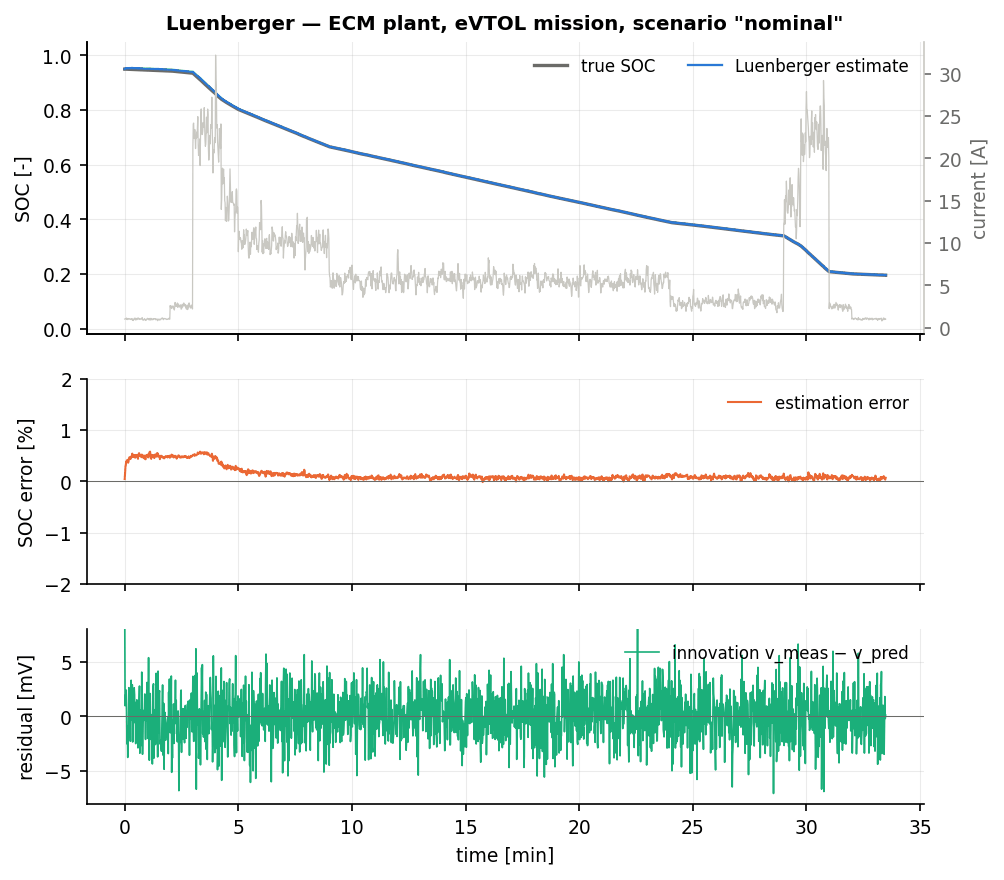
\includegraphics[width=\textwidth]{figures/cell_Luenberger_nominal.png}
\caption{Luenberger on the nominal eVTOL mission: true and estimated SOC (top), estimation error with the $\pm 2\sigma$ band when available (middle), voltage residual (bottom).}
\end{figure}
\begin{figure}[H]\centering
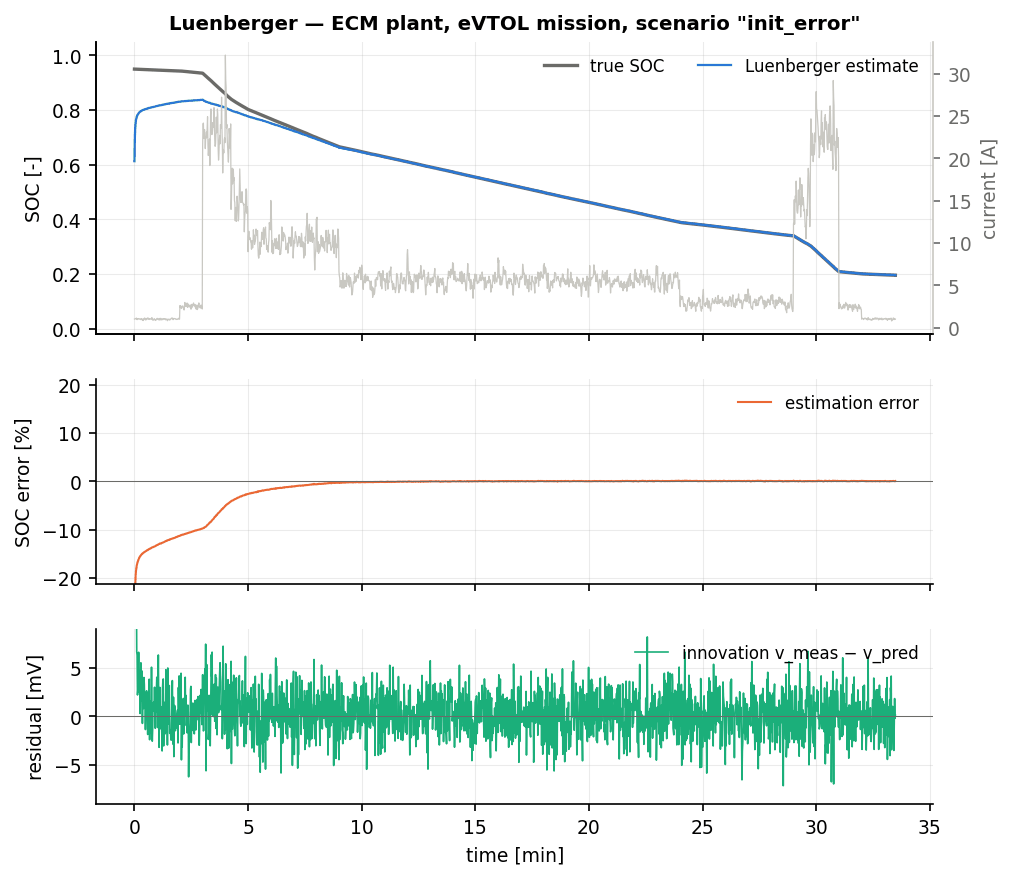
\includegraphics[width=\textwidth]{figures/cell_Luenberger_init_error.png}
\caption{Luenberger with a 35\,\% initial SOC error.}
\end{figure}

All numbers below are over three seeds; the spread is quoted whenever it is not negligible.  On
the nominal eVTOL mission the observer reaches $\mathrm{rmse}_{ss} = 0.0008$ SOC on every seed,
within a factor of two of the EKF's $0.0005$ and below the $0.02$ acceptance threshold by more
than an order of magnitude --- obtained without a covariance and at a third of the cost.  From a
$35\,\%$ initial error it converges in $334$\,s and settles to $0.0007$; the EKF converges faster
($0\,$s by the metric's definition) because its transient covariance gives it a large early gain,
which is precisely the advantage a fixed-gain observer gives up.

The scenario pattern follows the theory.  On \texttt{current\_bias} ($0.25$\,A offset plus a
$2\,\%$ gain error) the steady-state error is $0.0085$ against the EKF's $0.0061$: both are
dominated by \eqref{eq:lue-ssbias} with $\delta \approx R_0\Delta i \approx 4$\,mV, and no choice
of $\mL$ removes it.  On \texttt{param\_mismatch} ($R_0$ scaled by $0.7$) the observer gives
$0.0149$ versus the EKF's $0.0136$, and on \texttt{aged\_cell} $0.0218$ versus $0.0152$ --- again
the same mechanism.  \texttt{noise\_step} ($\sigma_v$ jumps to 20\,mV) barely moves the
Luenberger ($0.0033$) because a fixed gain cannot over-trust the measurement, whereas the
adaptive Kalman family has to detect the change first.  The most striking column is
\texttt{combined}, where the EKF reaches $\mathrm{rmse}_{ss}=0.1244$ and never converges, while
the Luenberger observer stays at $0.0213$ ($0.0204$--$0.0220$ across seeds) and converges in
$816$\,s: with four simultaneous faults the EKF's covariance is no longer a description of
anything, and a designed-bandwidth observer degrades far more gracefully than a mis-specified
optimal one.  The weakest columns are \texttt{aged\_cell} and \texttt{combined}, both limited by
\eqref{eq:lue-ssbias} rather than by the gain, and \texttt{preisach} ($0.0100$, where the
one-state hysteresis model is structurally wrong).

On the single-particle plant, where the estimator runs an ECM identified against a very different
model, the observer is at $0.0061$ on \texttt{nominal} and $0.0335$ on \texttt{cold} against the
EKF's $0.0373$ and $0.0735$ --- a factor of six and two respectively.  The ordering reverses
relative to the ECM plant for the same reason as \texttt{combined}: when the model is wrong the
optimal filter is optimal for the wrong problem.

\subsection*{How often is the placement actually used?}
The certification of \Cref{sec:lue-schedule} is not a formality.  Counting accepted placements
against total re-designs over the twelve ECM scenarios, the certified pole-placement gain is used
on $0/283$ re-designs on \texttt{nominal}, $0/331$ on \texttt{hot}, $0/420$ on
\texttt{param\_mismatch} and $0/445$ on \texttt{aged\_cell}, but $70$--$78$ of $\sim\!185$
($\approx 40\,\%$) on \texttt{cold} and $58$--$69$ of $\sim\!325$ ($\approx 20\,\%$) on
\texttt{combined}; the rest of the time the certified LQE gain is used instead.  The reason is
visible in the raw numbers: on \texttt{nominal} the placement gain achieves $\rho = 0.9986$ at the
frozen pair --- comfortably stable --- but $\rho = 1.0013$ to $1.0081$ over the family
\eqref{eq:lue-robust}, whereas the LQE gain achieves $0.9994$ to $0.9998$.  \emph{Exact
single-output pole placement is simply not robustly realisable on this plant at this sampling
rate}, and that is the honest headline of this chapter: the useful artefact is not the Ackermann
formula but the certification wrapper around it, which is what lets the same class carry a
placement design where one exists and an LQE design where one does not.  It also explains why
\texttt{Luenberger}, \texttt{HGO} and \texttt{SSKF} agree to three digits on most scenarios ---
they are running the same certified LQE gain --- and differ exactly on \texttt{cold}, where the
placement is admitted ($0.0040$ versus $0.0031$).

\section{Summary}
Use the Luenberger observer when the noise statistics are unknown or untrustworthy, when the
certification argument is about bounded convergence rather than optimality, or when the cycle
budget does not allow a covariance propagation.  Specify the poles as a repeated set, map them
from a time constant with $p=e^{-\dt/\tau}$, and validate every scheduled gain against a family
of perturbed linearisations rather than the frozen pair.  Do not use it when a calibrated
uncertainty output is required, when the measurement noise is genuinely non-stationary and you
want to exploit that, or when the dominant error is a persistent sensor bias --- for that,
continue to \Cref{ch:dob} or \Cref{ch:uio}.
